\chapter{Diseño e implementación}
\label{chap:diseño}

Este capítulo proporciona una visión detallada sobre la metodología y las herramientas utilizadas para medir el consumo energético y evaluar el rendimiento de modelos de aprendizaje automático en el contexto de la aplicación desarrollada: \texttt{MLCost}. Se comenzará describiendo la arquitectura de la aplicación y los módulos que la componen, para posteriormente profundizar en la metodología del proceso de aprendizaje. Este proceso empezará con la preparación de los datos, donde destacan las técnicas de preprocesamiento y la selección de modelos representativos de diversas familias algorítmicas. 

Durante la fase de entrenamiento, se empleará la biblioteca CodeCarbon para medir las emisiones de carbono y el consumo de energía, utilizando técnicas como la validación cruzada para evaluar la precisión y el rendimiento de los modelos. La evaluación de las predicciones se realiza a través de métricas estándar como precisión, exhaustividad y F-score, para obtener una estimación robusta del desempeño del modelo. Para finalizar, se presentarán los resultados con distintas herramientas de visualización y se discutirá la gestión eficaz de recursos, enfocándose en la configuración del procesador y el uso de múltiples núcleos para optimizar el rendimiento y minimizar el sesgo en las mediciones de consumo energético.


\section{Arquitectura}

\begin{figure}[H]
  \centerline{
     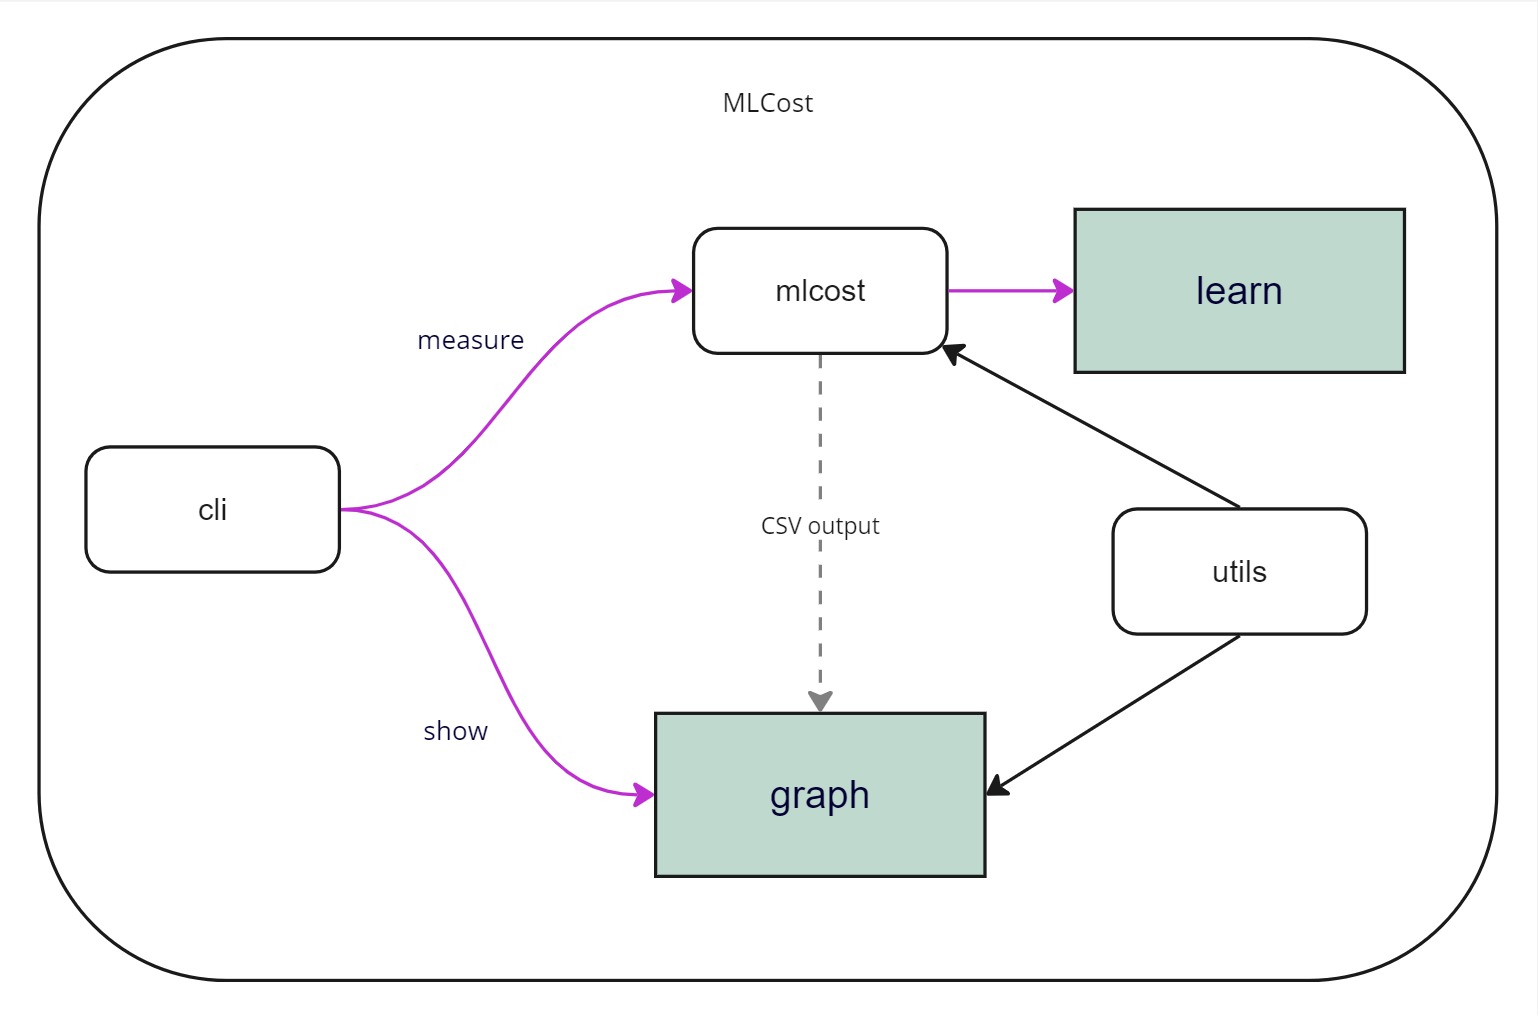
\includegraphics[width=\textwidth, keepaspectratio]{img/general-arch.jpg}
  }
  \caption{Arquitectura de la aplicación desarrollada}
  \label{fig:app-arch}
\end{figure}

La arquitectura de la aplicación se organiza en torno a varios componentes clave que se integran en el paquete \texttt{mlcost} para ofrecer un entorno robusto para la evaluación de modelos de aprendizaje automático en términos de precisión y eficiencia energética. 
%% info on packaging

El punto de entrada de la aplicación es el módulo \texttt{cli}, que se encarga de gestionar la interfaz de línea de comandos (\emph{command-line interface}, CLI) que facilita la interacción del usuario con las funcionalidades principales de la aplicación. Este módulo permite a los usuarios ejecutar la aplicación desde la terminal, proporcionando una manera flexible y accesible de realizar diversas operaciones, como la selección de modelos de aprendizaje automático, la configuración de parámetros de ejecución y la especificación de archivos de datos de entrada. El módulo \texttt{cli} utiliza la librería \texttt{click} para facilitar el procesamiento de los argumentos de la línea de comandos. Este enfoque permite definir una variedad de opciones y argumentos que los usuarios pueden especificar al ejecutar la aplicación. Por ejemplo, los usuarios pueden seleccionar que opciones de limpieza de datos serán utilizadas, establecer el número iteraciones para la validación cruzada, y decidir si serán ejecutadas en paralelo en el procesador. El conjunto completo de opciones de línea de comandos que se pueden utilizar está recogido en el Anexo~\ref{app:cli}. Una vez que se capturan los argumentos, \texttt{cli} invoca las funciones correspondientes definidas en el modulo \texttt{mlcost}.

Este modulo se encarga de la integración del seguimiento de emisiones de carbono y consumo energético durante el entrenamiento y la evaluación de los modelos de aprendizaje automático. Este módulo utiliza la biblioteca codecarbon para realizar el seguimiento del impacto ambiental de estos procesos computacionales. El módulo es responsable de gestionar el proceso de entrenamiento, creando un objeto de la clase \texttt{Trainer} por cada modelo a evaluar y asegurándose de que los datos son preprocesados para mejorar la precisión del modelo. Una vez que los datos están preparados, el módulo comienza la medición de emisiones, encarga el entrenamiento del modelo y, al finalizar, detiene el rastreador de emisiones y recupera los datos finales de consumo. Estos datos incluyen la duración del seguimiento, el consumo energético y las emisiones equivalentes de carbono. Los resultados, junto con los datos de rendimiento obtenidos durante la validación del modelo, se registran en un archivo para posterior referencia.

El núcleo de la aplicación reside en el modulo \texttt{learn}, que expone la clase \texttt{Trainer} ya mencionada, donde se definen las tareas principales de carga de datos, entrenamiento y evaluación de modelos, así como la recopilación de métricas de desempeño. Estos procesos serán descritos en mayor detalle en las secciones posteriores.

Para finalizar, la aplicación contiene dos módulos auxiliares que facilitan el desarrollo y proporcionan utilidades para examinar los resultados obtenidos.

El modulo \texttt{graphs} maneja la visualización de los resultados mediante diversas funciones de creación de gráficas que utilizan la librería matplotlib para crear gráficos de dispersión, de líneas y de barras. Estas visualizaciones ayudan a interpretar las relaciones entre las emisiones, el consumo de energía y las métricas de rendimiento de los modelos evaluados. Las gráficas también permiten comparar el desempeño de diferentes modelos bajo diversas cargas de CPU, ofreciendo una visión clara de cómo los recursos del sistema afectan la eficiencia y la precisión del modelo.

El componente \texttt{utils} proporciona funciones auxiliares para la aplicación, tales como la impresión de resultados y la recopilación de información del sistema operativo, así como la gestión de archivos de salida en formato CSV. Este archivo incluye utilidades para manejar los datos de emisiones y consumo energético, formateando la información de manera que sea fácilmente interpretable. 


\section{Lectura y limpieza de los datos}
\label{sec:limpieza}

El componente más importante de todo proyecto de aprendizaje automático son sin duda los datos. Por este motivo se han desarrollado con el tiempo una gran cantidad de librerías para facilitar la tarea de los desarrolladores que quieren trabajar con información de forma estructurada. En Python una de las más importantes es la librería \texttt{pandas} (\ref{sec:sota}), que ofrece la clase \texttt{DataFrame} con la que se pueden procesar grandes cantidades de datos de forma similar a como se trabajaría con una tabla o hoja de cálculo, con filas y columnas con distintos tipos de información.

Los conjuntos de datos que están disponibles de forma libre en repositorios de universidades y otras organizaciones de ciencia de datos no siempre siguen un mismo formato. Por este motivo el primer paso para aplicar métodos de aprendizaje automático en datos específicos será siempre deshacerse del formato de presentación y guardarlos en estructuras de datos operables por un ordenador, como \texttt{DataFrames} de \texttt{pandas}. En este proyecto, la intención ha sido ser capaz de procesar datos presentados con varios formatos distintos. Para ello, se han creado distintas argumentos para la línea de comandos que pueden ser utilizados al lanzar la aplicación especificando las características concretas del conjunto de datos a tratar.

En general, el proceso de lectura y limpieza de los datos va seguir siempre las siguientes fases:
\begin{enumerate}
    \item Lectura
    \begin{enumerate}
        \item Leer el archivo que contiene los datos.
        \item Separar los datos de entrenamiento de los datos de testeo.
        \item Identificar el tipo de datos de cada columna.
    \end{enumerate}
    \item Limpieza
    \begin{enumerate}
        \item Eliminar columnas que no pueden ser utilizadas.
        \item Reemplazar valores numéricos que falten.
        \item Reemplazar columnas categóricas por columnas booleanas.
        \item Escalar las características numéricas.
    \end{enumerate}
\end{enumerate}

El primer paso es leer los datos de uno o varios archivos, que serán generalmente archivos de texto en formato \texttt{.txt} o \texttt{.csv}. Es en este paso en el que se dan mayores diferencias entre distintos conjuntos de datos y la razón de que se hayan añadido las distintas opciones de línea de comandos al programa para resolverlo. Los archivos de texto que contienen los datos pueden utilizar diferentes caracteres separadores entre columnas (como coma o espacio), representar valores que no han sido tomados con diferentes símbolos (como '?' o '-'), presentar o no una fila inicial con los nombres de las columnas, identificar la columna de las etiquetas de distintas maneras e incluso separar en distintos archivos los conjuntos de entrenamiento y de testeo de forma previa. Todas estas opciones son tenidas en cuenta durante la lectura para convertir los archivos de texto en \texttt{dataframes} sobre los que las librerías de aprendizaje pueden operar. En el Anexo~\ref{app:cli} se incluye un compendio de todas las opciones disponibles en la aplicación.

Una vez que los datos están recogidos, el siguiente paso es separar los datos de entrenamiento de los de testeo. Para ello, primero se descartarán todas las filas de datos que no estén etiquetadas, si las hubiera. Por defecto, la separación se hace al 80-20 y de forma aleatoria, excepto si los conjuntos están previamente separados en dos archivos. Para terminar el proceso de lectura, las columnas que contienen características numéricas se separan de las que contienen características categóricas, para poder tratarlas de forma específica durante la limpieza.

En la sección de limpieza, el objetivo es eliminar las características que puedan crear obstáculos en el entrenamiento de los modelos. Tres problemas básicos son tratados: falta de datos en columnas numéricas, datos presentados de forma categórica y diferentes escalas de los datos numéricos. Para lidiar con ello se utilizará un tipo de clases provistas por la librería \texttt{scikit-learn} denominadas transformadores. Estos transformadores encapsulan distintas herramientas de preprocesado y limpieza que son usadas a menudo. Para la falta de datos numéricos, se utilizara un introductor simple de medidas (\texttt{SimpleImputer}), que rellenará los datos que falten con la media de los datos disponibles. 

Respecto a las columnas categóricas, muchos algoritmos de aprendizaje no están diseñados para trabajar directamente con variables no numéricas (generalmente, porque limitaría la eficiencia de los algoritmos). Para resolverlo, se utilizará un transformador denominado \texttt{OneHotEncoder}. Este transformador reemplaza una característica categórica con varias características booleanas, de forma que para cada posible valor de la categoría se crea una nueva columna con un valor de sí o no dependiendo de a cual pertenece cada dato. Para simplificar, características categóricas con más de diez valores distintos posibles serán descartadas completamente. Lo mismo ocurrirá con cualquier otra columna que no pueda ser identificada como numérica o categórica y con las filas en las que falten datos de tipo categórico.

Un último transformador, \texttt{StandardScaler}, será aplicado a las características numéricas para alinear la escala de todas ellas mediante una técnica denominada normalización de características. Este proceso consiste en transformar las características numéricas para que se sitúen dentro de un rango común, generalmente entre 0 y 1 o para que tengan media cero y varianza uno, como se hace con el \texttt{StandardScaler}. Esto ayuda a obtener mejores resultados en los modelos de aprendizaje automático por dos razones. Primero, evita que características con valores grandes dominen a aquellas con valores más pequeños, asegurando que todas las características contribuyan de manera equitativa al modelo. Segundo, algunos algoritmos, como los basados en distancias (por ejemplo, vecinos más cercanos o máquinas de vector soporte), funcionan mejor y convergen más rápido cuando las características están en la misma escala.


\section{Entrenamiento}

Una vez que los datos están preparados para su uso comienza la fase de entrenamiento. En este proyecto, el objetivo es medir el gasto energético de distintos modelos y compararlo con la calidad de sus predicciones. Para ello, se han elegido una serie de modelos representativos de las familias de algoritmos más utilizadas. Estos modelos elegidos serán entrenados uno detrás de otro con el conjunto de datos preparado mientras se mide el consumo energético mediante las herramientas proporcionadas por CodeCarbon.

El procedimiento es sencillo. En primer lugar se comienzan las mediciones mediante la creación se un objeto de tipo \texttt{EmissionsTracker} que cuenta con simples métodos \texttt{start()} y \texttt{stop()}. A continuación, se entrena el modelo en la parte del conjunto de datos reservada para entrenamiento, y seguidamente se aplica el modelo entrenado a la parte del conjunto de datos reservada para testeo para intentar predecir correctamente la etiqueta de cada entrada que contiene. Para finalizar, se detiene la medición de emisiones y se almacenan los resultados obtenidos.


\subsection{Modelos escogidos}
\label{subsec:models-short}

Dentro de los modelos de aprendizaje automático existen numerosas clasificaciones de acuerdo al tipo de tareas a realizar y la naturaleza de los datos. Este proyecto se centrará en tareas de clasificación por aprendizaje supervisado. En este subgrupo, destacan una serie de familias de algoritmos que suelen obtener buenos resultados para una gran variedad de tipos de datos.
\begin{enumerate}
    \item Modelos lineales. Se trata de modelos sencillos, fáciles de interpretar y eficientes computacionalmente, que funcionan bien cuando las relaciones entre las características de entrada y la salida son aproximadamente lineales. Uno de sus modelos más representativos es el de regresión logística (ver \ref{subsec:model-linear}).
    \item Árboles decisores. Estos algoritmos pueden modelar relaciones complejas en los datos y lidiar con no linealidad. Dentro de esta familia destaca el modelo de Bosque Aleatorio, que agrega predicciones de varios árboles decisores para mejorar la robustez del modelo (ver \ref{subsec:model-random-forest}).
    \item Máquinas de vector soporte (\ref{subsec:model-svm}). Estos modelos son efectivos tanto en tareas de clasificación lineales como no lineales y destacan por su gran versatilidad. Funcionan de forma óptima en conjuntos de datos relativamente pequeños pero de gran complejidad.
    \item Vecinos más cercanos. Su máximo representante, k vecinos más cercanos (k-NN, ver \ref{subsec:model-neighbors}), es un algoritmo simple e intuitivo que se basa en buscar relaciones locales entre los datos y puede ser efectivo en tareas tanto de regresión como de clasificación.
    \item Naive Bayes (bayesiano ingenuo). Se trata de una familia de modelos que destaca por su gran eficiencia, especialmente frente a conjunto de datos de gran complejidad, y especialmente útil en tareas de clasificación de texto. El clasificador más representativo es el Naive Bayes gaussiano (\ref{subsec:model-naive-bayes}).
    \item Métodos de conjuntos (ensemble). Estos métodos combinan las características de múltiples modelos para intentar mejorar el desempeño total. Entre ellos destacan las máquinas de potenciación de gradiente, que construyen sólidos modelos predictivos de forma iterativa (ver \ref{subsec:model-gradient}).
    \item Redes neuronales. Las redes neuronales, especialmente los modelos de aprendizaje profundo como las redes neuronales profundas (Deep Neural Networks, DNN, ver \ref{subsec:model-neural}), pueden formar representaciones jerárquicas complejas a partir de los datos, y son especialmente efectivas en tareas que involucran grandes cantidades de datos con patrones complejos.
\end{enumerate}

En general, se espera que modelos de aprendizaje más complejos como los métodos de conjuntos, las redes neuronales y las máquinas de vector soporte produzcan mejores predicciones a cambio de un mayor gasto energético que otros modelos comparativamente más sencillos computacionalmente, como los modelos lineales, Naive Bayes y vecinos más cercanos. En el capitulo~\ref{chap:experimentos}, se analizará si los resultados obtenidos durante los experimentos se corresponden con esta aproximación teórica.


\section{Registro de resultados}

\subsection{Evaluación de las predicciones}
\label{sec:scoring}

Para poder obtener una medida de utilidad de los distintos modelos, es necesario evaluar la calidad de las predicciones que realizan. Existen dos métodos principales realizar esta evaluación. El primero y más sencillo consiste en aplicar la función de predicción del modelo a un subconjunto de muestras que hayan sido aisladas previamente para no formar parte del proceso de entrenamiento. Estas predicciones se comparan con las etiquetas correctas de las muestras para determinar si cada predicción ha sido acertada.
Cuatro resultados distintos son posibles por muestra y clase concreta: verdadero positivo (TP, identificada correctamente como perteneciente a la clase), falso positivo (FP, identificada incorrectamente como perteneciente a la clase), falso negativo (FN, identificada incorrectamente como no perteneciente a la clase), y verdadero negativo (TN, identificada correctamente como no perteneciente a la clase). Una forma común de visualizar estos resultados es mediante una matriz de confusión, como la mostrada en la figura~\ref{fig:confusion-matrix}.

\begin{figure}[H]
  \centerline{
     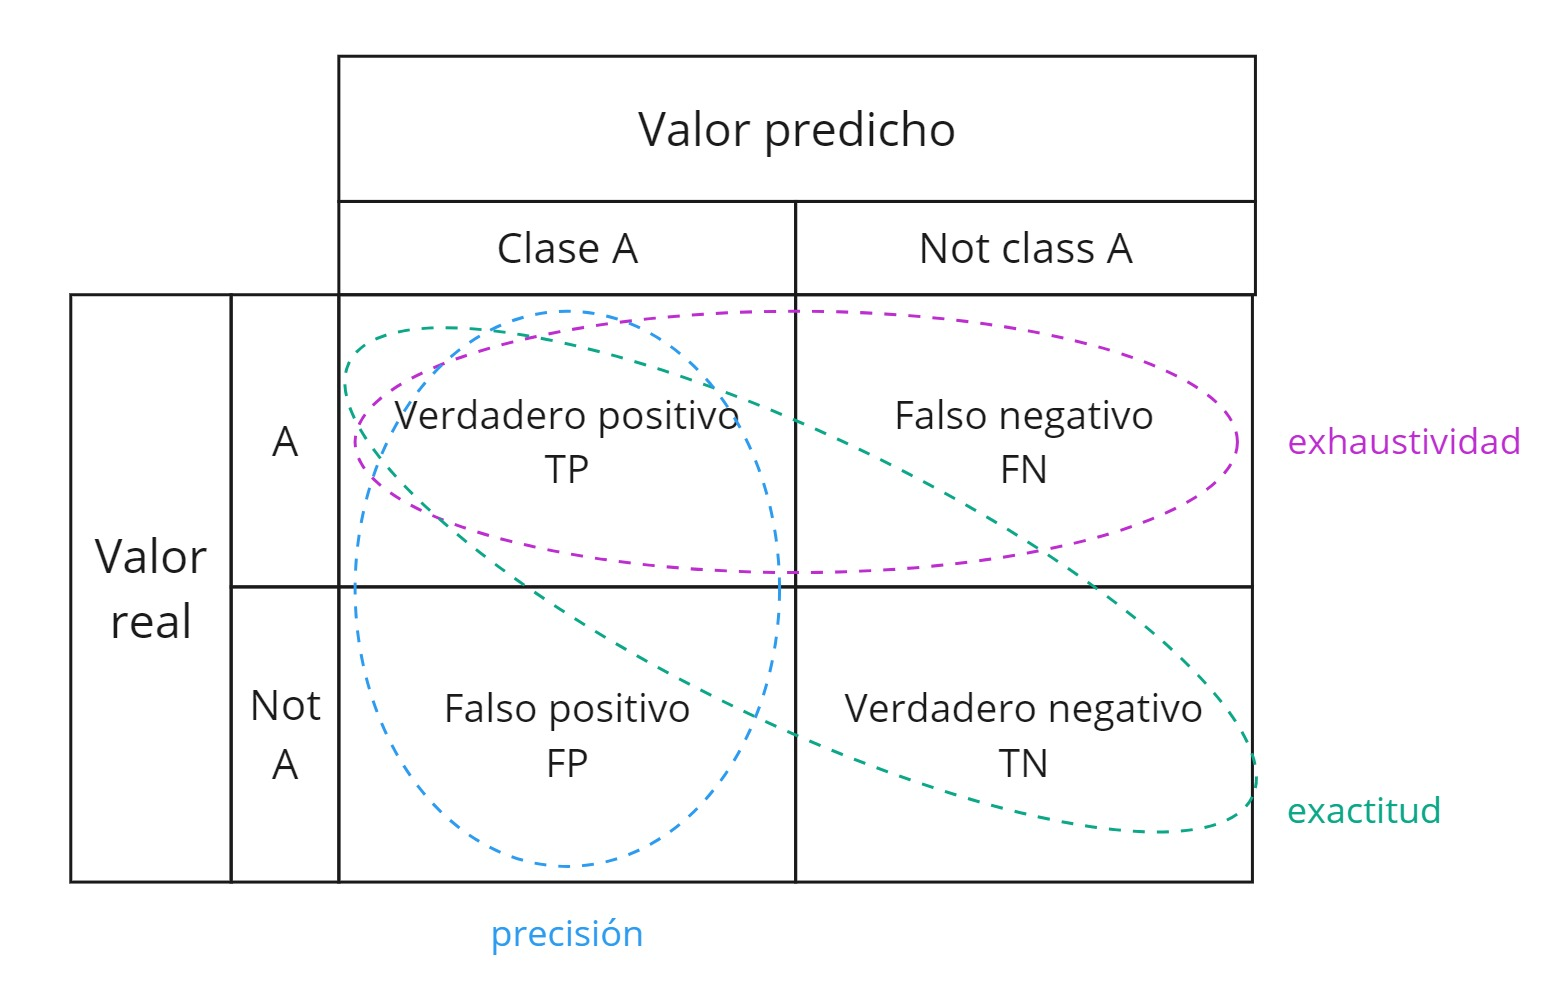
\includegraphics[width=0.8\textwidth, keepaspectratio]{img/confusion-matrix.jpg}
  }
  \caption{Matriz de confusión que muestra las relaciones entre posible resultados de la predicción.}
  \label{fig:confusion-matrix}
\end{figure}

A partir de las relaciones entre el número de muestras en cada uno de estos grupos se pueden extraer varias métricas del modelo, siendo las más comunes la exactitud, la precisión, la exhaustividad y el \emph{f-score}\cite{scikit-model-eval}. Estas métricas dan lugar a un valor entre 0 y 1, donde 0 es el peor resultado y 1 el mejor. También son comúnmente expresadas en porcentaje.

La \textbf{exactitud} (\emph{accuracy}) se define como la cercanía de la predicciones a su valor real. En tareas de clasificación se calcula como el número de predicciones correctas entre el número de muestras totales, como se puede ver en la ecuación \ref{eq:accuracy}. Una variante interesante de la exactitud que \texttt{scikit-learn} permite calcular es la exactitud balanceada, que evita medidas infladas de exactitud en conjuntos de datos no balanceados (con una o más clases sobrerrepresentadas en el conjunto) mediante la ponderación de cada muestra de acuerdo a la prevalencia inversa de su verdadera clase.

\begin{equation}
    a = \dfrac{TP+TN}{\text{muestras totales}}
\label{eq:accuracy}
\end{equation}

La \textbf{precisión} (\emph{precision}) y la \textbf{exhaustividad} (\emph{recall}) son métricas que analizan la relevancia de las muestras asignadas a cada clase y se calculan individualmente por clase. La precisión analiza el número de muestras correctamente clasificadas dentro de todas las muestras asignadas a una clase concreta, como muestra la ecuación \ref{eq:precision}, mientras que la exhaustividad analiza el número de muestras correctamente clasificadas en relación al número total de muestras reales existentes, como muestra la ecuación \ref{eq:recall}. Estas dos métricas pueden ser promediadas en función del peso relativo de cada clase un el conjunto para obtener una medida global de la precisión y exhaustividad del modelo.

\noindent
\begin{tabular}{@{}p{.4\linewidth}@{}p{.6\linewidth}@{}}
  \begin{equation}
     p = \dfrac{TP}{TP + FP}
  \label{eq:precision}
  \end{equation}
  &
  \begin{equation}
    r = \dfrac{TP}{TP + FN}
  \label{eq:recall}
  \end{equation}
\end{tabular}

En último lugar, es interesante mencionar el valor-F (\emph{F-score}), que se puede interpretar como una media harmónica de la precisión y la exhaustividad y tiene distintas variantes dependiendo de la importancia relativa de estas dos medidas. La denominada medida-$F_1$ da la misma importancia a la precisión y a la exhaustividad. Para cada clase, se calcula como muestra la ecuación \ref{eq:f-score}.

\begin{equation}
    F_1 = \dfrac{2\cdot TP}{2TP + FP + FN} = \dfrac{2pr}{p+r}
\label{eq:f-score}
\end{equation}

Estas cuatro medidas son calculadas por defecto en la aplicación desarrollada para todos los modelos entrenados. Para todos los casos, se utiliza la opción de scikit-learn \texttt{average='weighted'} para obtener las medidas, de forma que se puedan obtener valores más realistas en conjuntos con clases no balanceadas.

\subsubsection{Validación cruzada}

La aplicación desarrollada ofrece un segundo método para evaluar el rendimiento de un modelo mediante validación cruzada. Este método se basa en las mismas métricas ya mencionadas, pero con la peculiaridad de que éste se entrena varias veces de forma sucesiva con distintas distribuciones de los datos en un conjunto de entrenamiento y un conjunto de prueba. Posteriormente, se puede analizar la media y la desviación estándar de las métricas de la calidad de las predicciones obtenidas para cada distribución de las muestras y así obtener una idea más exacta del desempeño del modelo. En \texttt{scikit-learn}, la validación cruzada se puede implementar mediante el uso de la clase \texttt{KFold}, que divide el conjunto de datos en un número de pliegues especificados de forma aleatoria, y la función \texttt{cross\_validate}, que entrena el modelo y calcula las métricas deseadas para cada uno de los pliegues de forma sucesiva. Para determinar los plieges, la aplicación MLCost utiliza una clase derivada llamada \texttt{StratifiedKFold}, que ayuda a mantener el mismo ratio de muestras por clase en cada pliegue para conjuntos de datos no balanceados.

La validación cruzada ofrece varias ventajas significativas al evaluar el rendimiento de un modelo de aprendizaje automático. Una de las principales ventajas es que proporciona una estimación más robusta y fiable del desempeño del modelo al utilizar diferentes subconjuntos del conjunto de datos para entrenamiento y prueba en cada iteración. Esto ayuda a mitigar el riesgo de sobreajuste y ofrece una visión más generalizada de cómo se comportará el modelo con datos no vistos. Además, calcular la media y la desviación estándar de las métricas a través de los distintos pliegues permite una evaluación más precisa y detallada, identificando variaciones y asegurando que el modelo no solo es preciso sino también consistente.

Sin embargo, la validación cruzada también tiene desventajas. Uno de los principales inconvenientes es el aumento significativo en el tiempo de cómputo, ya que el modelo debe entrenarse y evaluarse múltiples veces, lo cual puede ser particularmente costoso en términos de tiempo y consumo energético, especialmente para conjuntos de datos grandes o modelos complejos. La utilización de un entorno de paralelización puede mitigar esta desventaja al permitir que los pliegues se procesen en paralelo, reduciendo así el tiempo total necesario para completar la validación cruzada. No obstante, la paralelización puede no ser igualmente efectiva en todos los tipos de hardware. Además, en entornos compartidos o con recursos limitados, la paralelización podría causar conflictos de recursos, afectando negativamente el rendimiento global del sistema. Por lo tanto, aunque la paralelización puede acelerar significativamente la validación cruzada, es crucial evaluar su uso en conjunción con las capacidades y limitaciones del hardware disponible. Este efecto será examinado durante las pruebas llevadas a cabo en la sección~\ref{sec:test-2-resources}.


\subsection{Medición de emisiones}

Durante la ejecución de su rastreador de emisiones, la librería CodeCarbon calcula varias medidas distintas para identificar el consumo energético. En primer lugar, las emisiones están geolocalizadas de una de las siguientes formas: mediante una conexión a internet automática que permita identificar la localización mediante rastreo de IP, o mediante la especificación de un país determinado en el código al crear el objeto rastreador de emisiones. Esta localización es necesaria para convertir los kilovatios consumidos durante el proceso de entrenamiento en emisiones de carbono equivalentes, que dependerán de la mezcla especifica de producción de energía que haya establecido cada país. De esta forma, si la energía estuviera producida en gran medida por energías renovables, las emisiones de carbono serían mucho menores que si la energía fuera producida en su totalidad en una planta de quema de carbón. En la sección de resultados se compararán las diferencias de emisiones producidas entrenando modelos en un mismo conjunto de datos en diferentes localizaciones.

Con estos datos, la librería CodeCarbon calcula las emisiones a partir de medidas de la capacidad del procesador y gráfica de la máquina, del porcentaje de su uso que corresponde al proceso de entrenamiento observado y de la duración total del proceso. En este proyecto, por cada modelo entrenado se guardan tres de estas medidas para su posterior análisis y comparativa: la energía consumida (en kilovatios hora, \unit{kWh}), las emisiones calculadas (en kilogramos equivalentes de carbono, $\unit{kg\;[CO_2eq]}$]) y la duración (en segundos). Durante el proceso de entrenamiento, estos valores son escritos en un archivo de texto de tipo CSV (\emph{comma-separated values}) junto con las medidas de calificación de las predicciones mencionadas en el apartado anterior. Este archivo de texto será utilizado posteriormente para dibujar gráficas de las que extraer conclusiones con una herramienta de gráficos desarrollada para este proyecto.


\subsection{Herramientas de visualización}

La visualización de los resultados obtenidos es crucial para interpretar y analizar las métricas de consumo energético y rendimiento de los modelos de aprendizaje automático evaluados. A través de gráficos, es posible identificar patrones, tendencias y relaciones entre distintas variables que de otra manera serían difíciles de detectar en tablas de datos. Esto facilita la toma de decisiones informadas y permite comunicar los hallazgos de manera más efectiva.

El motor de gráficos utilizado en este proyecto es Matplotlib (ver \ref{subsec:matplotlib}, una biblioteca de Python ampliamente utilizada para la creación de gráficos estáticos, animados e interactivos. Matplotlib proporciona una gran flexibilidad y control sobre la generación de gráficos, permitiendo a los desarrolladores personalizar todos los aspectos visuales de sus representaciones gráficas.

Para generar los gráficos, es necesario haber ejecutado previamente una medición de emisiones con la opción \texttt{--log} activada. Esto crea un archivo CSV que contiene los datos recopilados durante las pruebas, incluyendo métricas de rendimiento y consumo energético. Este archivo CSV es esencial para la visualización, ya que contiene toda la información requerida para producir los gráficos. Los gráficos se generan utilizando el comando \texttt{mlcost show -f <output-file.csv>}. Este comando lee el archivo CSV especificado y produce una variedad de gráficos que ayudan a visualizar los resultados de las pruebas.

El módulo \texttt{graph} incluye varias funciones auxiliares para la creación de diferentes tipos de gráficos. Entre ellas se encuentran funciones para generar gráficos de dispersión con tres o cuatro variables, así como gráficos de líneas y barras. Las funciones de dispersión permiten comparar variables como emisiones y precisión a través de diferentes modelos y conjuntos de datos, utilizando diferentes marcadores y colores para distinguir entre categorías. Por otro lado, los gráficos de líneas y barras se utilizan para visualizar tendencias y comparaciones categóricas, aprovechando las capacidades de la librería Pandas para agrupar los datos recogidos en \texttt{DataFrames} y producir gráficas con ellos de manera eficiente.

\section{Gestión de recursos}

Un aspecto importante para obtener mediciones precisas del consumo energético y del rendimiento de los modelos de aprendizaje automático es la gestión de los recursos disponibles en la máquina que está tomando las medidas. Los resultados obtenidos por la librería CodeCarbon para estimar el consumo eléctrico se basan en el modelo y el tiempo de utilización del procesador. De esta forma, CodeCarbon rastrea el uso de recursos durante el entrenamiento de los modelos y calcula las emisiones de $CO_2$ correspondientes.

La carga del procesador en el momento de tomar las medidas de consumo energético es un factor crucial. Una alta carga del procesador puede indicar que el sistema está ejecutando múltiples tareas simultáneamente, lo cual puede sesgar los resultados. Para mitigar este efecto, CodeCarbon intenta aislar el proceso de aprendizaje del resto de tareas del ordenador al utilizar la opción {\texttt{tracking\_mode="process"} en su clase medidora de emisiones \texttt{EmissionTracker}. Esta opción permite que la herramienta enfoque la toma de medidas en el proceso específico que se está evaluando, minimizando la interferencia de otras operaciones del sistema. 

Sin embargo, este enfoque añade una capa adicional de aproximación al cálculo de emisiones, por lo que para obtener medidas más consistentes será interesante mantener una carga baja del procesador al comenzar el proceso. Al inicio de la aplicación, ésta imprime al terminal tanto la información del sistema y del modelo del procesador como su carga de trabajo inicial en porcentaje de utilización. Además, el archivo de datos recopilados generado por el programa contiene una columna con la carga al finalizar el entrenamiento de cada modelo. Una carga baja al comienzo del experimento significará que la máquina no está realizando otras tareas pesadas que podrían influir en las mediciones de consumo energético y rendimiento. Esto ayudará a que los datos reflejen de manera más precisa el impacto del entrenamiento del modelo en el consumo energético.


\subsection{Procesamiento multinúcleo}

El uso de ordenadores con varios núcleos en el procesador o de varios procesadores asignados a la misma tarea puede afectar tanto al rendimiento como a las emisiones. En términos de rendimiento, la capacidad de realizar múltiples tareas simultáneamente (\emph{multitasking}) permite que los modelos se entrenen más rápido, ya que pueden aprovechar el paralelismo inherente a muchos de los algoritmos de aprendizaje automático. Sin embargo, esta mejora en el rendimiento puede venir acompañada de un aumento en el consumo energético, ya que más núcleos en uso implican un mayor consumo de energía.

La biblioteca scikit-learn gestiona el paralelismo a través del parámetro \texttt{n\_jobs}, el cual se puede especificar en diversas funciones y modelos para indicar el número de procesos paralelos que se deben utilizar. La aplicación desarrollada acepta este parámetro al ejecutarla por línea de comandos y lo comunica a scikit-learn, permitiendo que se configure la cantidad de CPUs disponibles para ejecutar tareas en paralelo. Esta configuración puede reducir significativamente el tiempo de cómputo en experimentos de gran escala.

Internamente, scikit-learn utiliza el contexto {joblib.parallel\_backend} para gestionar el paralelismo. {joblib.parallel\_backend} es una función que permite seleccionar el backend de paralelización que se utilizará durante la ejecución de las operaciones paralelas. El backend de joblib puede manejar diferentes tipos de paralelismo, como threading y multiprocessing, adaptándose a las características del hardware y a las necesidades del usuario. Cuando se especifica \texttt{n\_jobs}, {joblib.parallel\_backend} se encarga de dividir las tareas entre los procesos disponibles y de gestionar la sincronización y la recolección de resultados.

Dentro del proceso de aprendizaje, hay varias funciones en las que scikit-learn ofrece la posibilidad de ejecutar tareas en paralelo. Una de ellas es la validación cruzada, que es particularmente adecuada para la paralelización, ya que cada pliegue del conjunto de datos puede ser procesado de manera independiente. Por otra parte, varios modelos pueden ser entrenados directamente en paralelo dentro de una única iteración especificando el número de procesos a utilizar. Entre los modelos que admiten \texttt{n\_jobs} se encuentran el bosque aleatorio, las máquinas de potenciación de gradiente, y vecinos más cercanos. Sin embargo, otros modelos como los lineales, las máquinas de vector soporte, Naive Bayes, y las redes neuronales no siempre permiten especificar un número de procesos en paralelo de forma nativa.

Para lidiar con estas diferencias, la aplicación desarrollada se limita a aplicar el número de procesos únicamente a la validación cruzada y no al entrenamiento directo de los modelos. Esta decisión se toma para poder comparar todos los modelos en igualdad de condiciones. De esta forma, se asegura que cualquier mejora en el tiempo de ejecución sea atribuible únicamente a la paralelización del proceso de validación cruzada y no a diferencias intrínsecas en la implementación de cada modelo.

El efecto que la paralelización y la gestión de los recursos de la máquina donde se realiza el entrenamiento se podrá observar en el experimento de la sección \ref{sec:test-2-resources}. En esta prueba, 
se entrenarán los modelos en diferentes máquinas virtuales desplegadas en Microsoft Azure, cada una con configuraciones de procesador y memoria RAM distintas y alternando entre utilizar paralelización o no durante el entrenamiento. Este experimento permitirá estudiar los resultados de emplear varios procesadores en el entrenamiento por validación cruzada, analizando cómo el paralelismo y la configuración de hardware afectan tanto al rendimiento de los modelos como al consumo energético.

% \todoin{TO-DO EXPLICAR \\
% > Azure deployment
% > plantillas }

\clearpage